
\newcommand{\titleinfo}{Leistungselektronik  - Formelsammlung}
\newcommand{\authorinfo}{S\"ami Bertsch}
\newcommand{\versioninfo}{ }

\include{./header/header}



%%%%%%%%%%%%%%%%%%%%%%%%%%%%
% Mathematische Operatoren %
%%%%%%%%%%%%%%%%%%%%%%%%%%%%

\newcommand{\zaehlerBuck}{\frac{1}{i_{Lmax}} \cdot \frac{V_{1}}{R_{1}} - 1   }
\newcommand{\nennerBuck}{\frac{1}{i_{Lmax}} \cdot \frac{V_{1}}{R_{1}}-e^{\frac{-T_{a}}{\tau}} }

\begin{document}

\section{Allgemeine Formeln}

\begin{tabu}{|l|l|}
	\hline
  Spannung über einer Induktivität
  	&\ $u_{L}(t) = L\frac{di}{dt}$\\
	\hline
  Strom durch Kondensator 
  	&\ $i_{C}(t) = C\frac{du}{dt}$\\
  	\hline
  Zeitkonstante $\tau$
  	&\ $\tau = \frac{L}{R}$ oder $\tau = RC$\\
  	\hline
  Berechnung des Mittelwertes
  	&\ $X_{AV} = \frac{1}{T}\int\limits_{0}^{T}x(t)dt$\\
  	\hline
  Berechnung des Gleichwertes
  	&\ $\overline{|X|} = \frac{1}{T} \int\limits_{0}^{T} |x(t)|dt$\\
  	\hline
  Berechnung des Effektivwertes
  	&\ $X_{RMS} = \sqrt{\frac{1}{T}\int\limits_{0}^{T}x^2(t)dt}$\\
  	\hline
  Effektivwert Oberwellen
    & $X_{RMS\_Oberwellen} = \sqrt{X_{RMS}^2 - X_{AV}^2}$\\
  \hline
  Formfaktor
    & $F = \frac{X_{RMS}}{\overline{|X|}}$\\
  \hline
  Welligkeit
  	& $w = \frac{X_{RMS\_Oberwellen}}{|X_{AV}|}= \frac{\sqrt{\sum\limits_{k = 1}^{\infty}X_{k}^2}}{|X_{AV}|} = \sqrt{F^2-1}$\\
  \hline
\end{tabu}

\section{Berechnung der höheren Harmonischen}
\subsection{Orthogonalitätsbeziehungen}


            $\int\limits_0^T \cos(n\omega t)\cdot \cos(m\omega t)dt=
            \begin{cases}
            T,\ n=m=0\\
            \frac{T}{2},\ n=m>0\\ 
            0,\ n\neq m\\
            \end{cases}$\\
            
            
           $\int\limits_0^T \sin(n\omega t)\cdot \sin(m\omega t)dt=
           \begin{cases}
           \frac{T}{2},\ n=m\\
           0,\ n\neq m\\
           \end{cases}$\\
           $\int\limits_0^T \cos(n\omega t)\cdot \sin(m\omega t)dt=0$
           
\subsection{Allgemeine Form}
Eine periodische Funktion lässt sich durch eine Reihe von Sinus- und Kosinusfunktionen darstellen.
$$f(t) = \frac{a_{0}}{2}+\sum_{n = 1}^{\infty} (a_{n} \cdot cos(n \omega t)+ b_{n} \cdot sin(n \omega t))$$

Die Koeffizienten der Entwicklung von $f(t)$ sind:\\
\begin{tabular}{ll}
  $a_{n} = \frac{2}{T}\int_{0}^{T}f(t) \cdot cos(n \omega t)dt$   &\ $(n = 0,1,2,...)$\\
  $b_{n} = \frac{2}{T}\int_{0}^{T}f(t) \cdot sin(n \omega t)dt$   &\ $(n = 1,2,3,...)$\\
\end{tabular}
\subsection{Sätze zur Berechnung der Koeffizienten}
\subsubsection{Symmetrie}
\begin{tabular}{ll}
  Falls $f(t)$ gerade ist $(f(t) = f(-t))$: &\ $\rightarrow b_{n} = 0, a_{n} = \frac{4}{T}\int_{0}^{\frac{T}{2}} f(t) \cdot cos(n \omega t)dt$\\
  Falls $f(t)$ ungerade ist $(f(-t) = -f(t))$: &\ $\rightarrow a_{n} = 0, b_{n} = \frac{4}{T}\int_{0}^{\frac{T}{2}} f(t) \cdot sin(n \omega t)dt$\\
\end{tabular}\\\\
Beispiele von geraden Funktionen sind $x^2, cos(x)$ und Beispiele ungerader Funktionen sind $x, x^3, sin(x)$.


\section{Ungesteuerter Gleichrichter M1U}
\begin{tabular}{ll}
  Mittelwert &\ $U_{R AV} = \frac{1}{T}\int\limits_{0}^{T}u_{R}(t)dt = \frac{1}{2\pi}\int\limits_{0}^{\pi}U_{2m} \cdot sin(\alpha)d\alpha, \alpha = \omega t$\\
  &\ $U_{R AV} = -\frac{U_{2m}}{2\pi}(cos(\pi)-cos(0))= \frac{U_{2m}}{\pi}$\\
  bei f = 50 Hz&\ $U_{R AV} = \frac{1}{20 ms}\int\limits_{0}^{10 ms}u_{R}(t)dt, T = \frac{1}{f}$\\\\
  Effektivwert &\ $U_{R RMS} = \sqrt{\frac{1}{T}\int\limits_{0}^{T}u_{R}^2 \cdot dt} = \sqrt{\frac{1}{2\pi}\int\limits_{0}^{\pi}U_{2m}^2 \cdot sin^2(\alpha) \cdot d\alpha} = \frac{U_{2m}}{2}$\\
  allgemein &\ $\int\limits_{0}^{\pi}sin^2(\alpha) \cdot d\alpha = \frac{\pi}{2}$\\
  bei f = 50 Hz &\ $U_{R RMS} = \sqrt{\frac{1}{20 ms}\int\limits_{0}^{10 ms}u_{R}^2 \cdot dt}$\\\\
  Laststrom &\ $i_{R}(t) = \frac{u_{R}(t)}{R}$\\
  Wirkleistung &\ $P = \frac{1}{2\pi}\int\limits_{0}^{\pi}\frac{u_{R}^2(\alpha)}{R} \cdot d\alpha = \frac{U_{R RMS}^2}{R} = \frac{U_{2m}^2}{4R}$
\end{tabular}


\section{Gesteuerter Gleichrichter M1C}
der Steuerwinkel des Gleichrichter: $\alpha \in [0, \pi]$\\\\
\begin{tabular}{ll}
  Mittelwert &\ $U_{R AV} = \frac{1}{2\pi}\int_{\alpha}^{\pi}U_{2m} \cdot sin(\beta) \cdot d\beta, \beta = \omega t$\\
  &\ $U_{R AV} = \frac{U_{2m}}{2\pi}(1 + cos(\alpha))$\\\\
  Effektivwert &\ $\sqrt{\frac{U_{2m}^2}{2\pi}\int_{\alpha}^{\pi}sin(\beta)^2 \cdot d\beta} = U_{2m} \cdot \sqrt{\frac{\pi-\alpha}{4\pi}+\frac{sin(2\alpha)}{8\pi}}$\\
  allgemein &\ $\int_{\alpha}^{\pi}sin(\beta)^2 \cdot d\beta = \frac{\pi-\alpha}{2}+\frac{sin(2\alpha)}{4}$\\\\
\end{tabular}

\section{Gesteuerter Gleichrichter B2C}

\begin{tabu}{|l|l|p{0.3\textwidth}}
	\cline{1-2}
  Mittelwert 
  	&\ $\begin{aligned}
  			U_{R AV} &= \frac{1}{\pi}\int\limits_{\alpha}^{\pi}U_{2m} \cdot sin(\beta) \cdot d\beta, \qquad \beta = \omega t\\
  						&= \frac{U_{2m}}{\pi}(1 + cos(\alpha))
  		\end{aligned}$ 
  		& \multirow{2}{*}{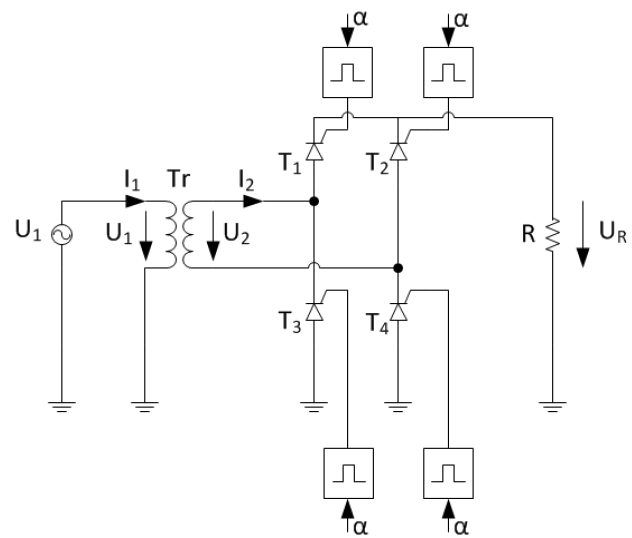
\includegraphics[width = \linewidth, height = 4cm]{./pictures/b2c.png}}\\
  \cline{1-2}
  Effektivwert 
  	&\ $\begin{aligned}
  		U_{R RMS} &= \sqrt{\frac{2 U_{2m}^2}{T}\cdot \int\limits_{a}^{\nicefrac{T}{2}} \sin^2\left( \frac{2\pi}{T} t\right) dt} = \left| \begin{aligned} \beta &= \frac{2\pi}{T}\cdot t \\ d\beta &= \frac{2\pi}{T} \cdot dt\end{aligned} \right| =\\
          &= \sqrt{\frac{U_{2m}^2}{\pi}\cdot\int\limits_{\alpha}^{\pi} \sin^2(\beta)d\beta} = U_{2m} \cdot \sqrt{\frac{\pi-\alpha}{2\pi}+\frac{sin(2\alpha)}{4\pi}}
  		\end{aligned}$ &\\
  \cline{1-2}
\end{tabu}

\section{Leistungsberechnung}
\begin{tabular}{|l|l|}
  \hline
  Momentane Leistung
  	& $p(t) = u_{R}(t) \cdot i_{R}(t)$\\
  \hline
  Wirkleistung
  	& $P = \frac{1}{2\pi}\int_{0}^{\pi}\frac{u_{R}^2(\alpha)}{R} \cdot d\alpha = \frac{U_{R RMS}^2}{R}$\\
  \hline
  Wirkleistung (Trafoseitig)
  	& $P = U \cdot I_{1} \cdot cos(\varphi_{1})$ \newline
  		dabei ist $I_{1}$ die erste Harmonische Komponente des Stromes \\
  		& und $\varphi_{1}$ die Phasenverschiebung \\
  \hline
  Grundschwingungsblindleistung
  	& $Q_{1} = U \cdot I_{1} \cdot sin(\varphi_{1})$\\
  \hline
  Verzerrungsleistung
  	& $Q_{V} =  U \cdot \sqrt{\sum_{k = 2}^{\infty}I_{k}^2}$\\
  \hline
  gesamte Blindleistung
  	& $Q = \sqrt{Q_{1}^2 + Q_{V}^2}$\\
  \hline
  Grundschwingungsscheinleistung
  	& $S_{1} = U \cdot I_{1}$\\
  \hline
  gesamte Scheinleistung
  	& $S = U \cdot I_{RMS} = \sqrt{P^2 + Q^2} = \sqrt{P^2 + Q_{1}^2 + Q_{V}^2}$\\
  \hline
  Leistungsfaktor
  	& $\lambda = \frac{P}{S}$\\
  \hline
  Welligkeit
  	& $w = \frac{F_{RMS}}{F_{AV}}= \frac{\sqrt{\sum_{k = 1}^{\infty}F_{k}^2}}{F_{AV}}$\\
  \hline
\end{tabular}

\section{Schaltverluste, Kühlung}
B2C als Beispiel:\\\\
in einem ersten Schritt muss der Strom durch den Thyristor berechnet werden:\\
\begin{tabular}{ll}
  &\ $I_{Rm} = \frac{U_{2m}}{R}$\\\\
  Mittelwert des Thyristorstroms &\ $I_{T AV} = \frac{1}{2\pi}\int_{\alpha}^{\pi}I_{Rm} \cdot sin(\beta) \cdot d\beta, \beta = \omega t$\\
  &\ $I_{T AV} = \frac{I_{Rm}}{2\pi} \cdot (1+cos\alpha)$\\\\
  Effektivwert des Thyristorstroms &\ $I_{T RMS} = \sqrt{\frac{I_{RM}^2}{2\pi}\int_{\alpha}^{\pi}sin^2(\beta)d\beta}$\\
  &\ $I_{T RMS} = \frac{I_{Rm}}{2}\sqrt{\frac{\pi - \alpha}{\pi}+\frac{sin2\alpha}{2\pi}}$\\\\
\end{tabular}

\begin{figure}[htbp]
  \begin{minipage}[t]{6cm}
    \vspace{0pt}
    \centering
    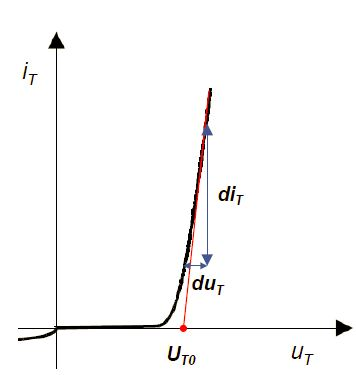
\includegraphics[width = 5cm]{./pictures/kennlinieThyristor} 
  \end{minipage}
  \hfill
  \begin{minipage}[t]{6cm}
    \vspace{0pt}
    Durchlassrichtung: $i_{T}, u_{T}$\\
    Schwellenspannung: $U_{T0}$\\
    Differentieller Durchlasswiderstand: $r_{T} = \dfrac{du_{T}}{di_{T}}$\\
    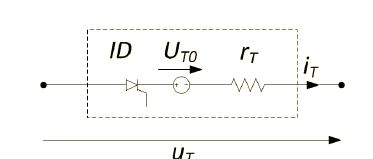
\includegraphics[width = 4cm]{./pictures/schemaThyristor}\\
    $u_{T} = U_{T0}+i_{T}(t) \cdot r_{T}$
  \end{minipage}
\end{figure}

momentane Verlustleistung: $p(t) = u_{T}(t) \cdot i_{T}(t)$\\
\begin{tabular}{ll}
  Mittelwert der Verlustleistung: &\ $P_{T} = \frac{1}{T}\int_{0}^{T}u_{T}(t) \cdot i_{T}(t) \cdot dt$\\
  &\ $P_{T} = U_{T0} \cdot \frac{1}{T}\int_{0}^{T}i_{T}(t)dt+r_{T} \cdot \frac{1}{T}\int_{0}^{T}i_{T}^2(t)dt$\\\\
  &\ $P_{T} = U_{T0} \cdot I_{T AV} + r_{T} \cdot I_{T RMS}^2$\\
  &\ $I_{T AV}$ ist der Mittelwert und $I_{T RMS}$ der\\ &\ Effektivwert des Thyristorstroms\\
\end{tabular}

\textbf{Die Werte für $U_{T0}$ können aus dem Datenblatt des Thyristors herausgelesen werden.}\\\\\\
\begin{tabular}{|l|l|}
  \hline
  \textbf{Thermische Kenngrössen} &\ \textbf{Elektrische Kenngrössen}\\
  \hline
  Wärmeleistung $ P (W) $ &\ Strom $ I (A) $\\
  \hline
  Temperaturunterschied $\vartheta (K)$ &\ Spannung $U (V)$\\
  \hline
  Wärmewiderstand $R_{th} (\frac{K}{W})$ &\ Widerstand $R (\frac{V}{A})$\\
  \hline
\end{tabular}

\subsection{Thyristor ohne Kühlkörper}
\begin{figure}[htbp]
  \begin{minipage}[t]{6cm}
    \vspace{0pt}
    \centering
    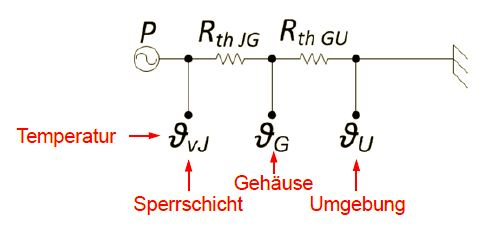
\includegraphics[width = 5cm]{./pictures/ohneKuehlkoerper} 
  \end{minipage}
  \hfill
  \begin{minipage}[t]{6cm}
    \vspace{0pt}
    $\vartheta_{vJ} - \vartheta_{U} = P \cdot (R_{th JG}+ R_{th GU})$\\
    $ \vartheta_{vj} = P \cdot (R_{th JG}+ R_{th GU}) + \vartheta_{U}$\\\\\\
    \textbf{$R_{th}$ muss wiederum aus dem Datenblatt herausgelesen werden.}
  \end{minipage}
\end{figure}

\subsection{Thyristor mit Kühlkörper}
\begin{figure}[htbp]
  \begin{minipage}[t]{6cm}
    \vspace{0pt}
    \centering
    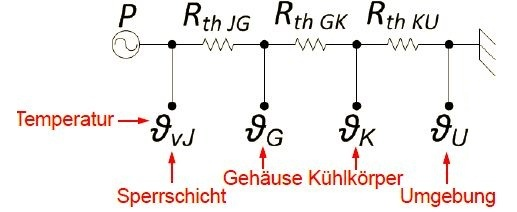
\includegraphics[width = 5cm]{./pictures/mitKuehlkoerper} 
  \end{minipage}
  \hfill
  \begin{minipage}[t]{6cm}
    \vspace{0pt}
    $\vartheta_{vJ} - \vartheta_{U} = P \cdot (R_{th JG}+ R_{th GK}+ R_{th KU})$\\
    $ \vartheta_{vj} = P \cdot (R_{th JG}+ R_{th Gk} +R_{th KU}) + \vartheta_{U}$\\\\\\
    
  \end{minipage}
\end{figure}


\section{Gleichstromumrichter}
\subsection{Buck-Converter (Tiefsetzsteller)}

Ein einfacher Tiefsetzsteller könnte auch mit einem Spannungsteiler bebaut werden.
Die Verlustleistung würde jedoch $P_{V} = R_{1} \cdot I_{1}^2$ betragen.


\begin{longtable}{|p{0.1\textwidth}|l|p{0.3\textwidth}}
	\cline{1-2}
	\multicolumn{2}{|c|}{\textbf{Grundgleichungen}}
	& \multirow{3}{*}{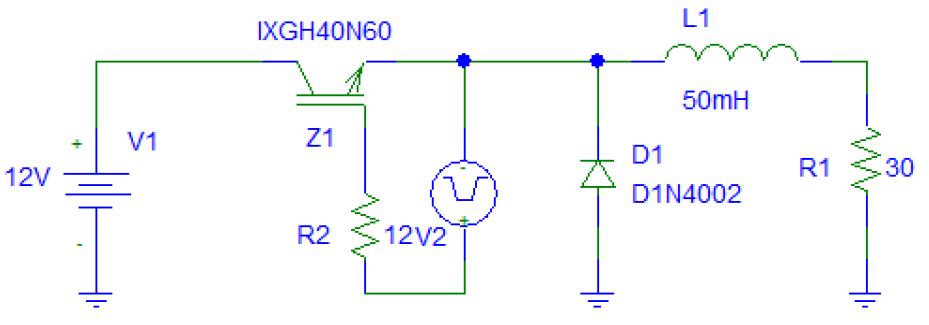
\includegraphics[width = \linewidth]{./pictures/buck.png}}\\
	\cline{1-2}
	DGL
		& $\begin{aligned}
			& i_{L} \cdot R + L\dfrac{di_{L}}{dt} = U_1  & t \in [0; T_{e}]\\
			& i_{L} \cdot R + L\dfrac{di_{L}}{dt} = 0  & t \in [T_{e}; T_{s}]
		\end{aligned}$ & \\[5mm]
	\cline{1-2}
	Stromverlauf (Lösung der DGL)
		& $i_L = \begin{cases}
					\frac{V_{1}}{R_{1}}+\frac{V_{1}}{R_{1}} \cdot \frac{-1+e^{\frac{-T_{a}}{\tau}}}{1-e^{\frac{-T_{s}}{\tau}}} \cdot e^{\frac{-t}{\tau}} & t \in [0; T_{e}]\\
					\frac{V_{1}}{R_{1}} \cdot \frac{1-e^{\frac{-T_{e}}{\tau}}}{1-e^{\frac{-T_{s}}{\tau}}} \cdot e^{\frac{-(t+T_{e})}{\tau}} & t \in [T_{e}; T_{s}]
			\end{cases}\quad \text{mit} \quad \tau = \frac{L_{1}}{R_{1}}$& \\
	\cline{1-2}
	Ein- und Ausschaltzeiten
		& $\begin{aligned}
			T_{a} &= -\tau \cdot \ln\frac{i_{Lmin}}{i_{Lmax}}\\
			T_{e} &= -\tau \cdot \ln\left(\frac{\zaehlerBuck}{\nennerBuck}\right)\\
			T_{s} &= T_{e} + T_{a}\\
			\tau &= \frac{L_{1}}{R_{1}}
		\end{aligned}$ &\\
	\cline{1-2}
\end{longtable}


\input{./sections/gleichstromschalter}

\end{document}